% Options for packages loaded elsewhere
\PassOptionsToPackage{unicode}{hyperref}
\PassOptionsToPackage{hyphens}{url}
%
\documentclass[
]{article}
\title{In what trauma patient subgroups are oppotunities for improvement
most frequent?}
\author{George Sandelswärd}
\date{}

\usepackage{amsmath,amssymb}
\usepackage{lmodern}
\usepackage{iftex}
\ifPDFTeX
  \usepackage[T1]{fontenc}
  \usepackage[utf8]{inputenc}
  \usepackage{textcomp} % provide euro and other symbols
\else % if luatex or xetex
  \usepackage{unicode-math}
  \defaultfontfeatures{Scale=MatchLowercase}
  \defaultfontfeatures[\rmfamily]{Ligatures=TeX,Scale=1}
\fi
% Use upquote if available, for straight quotes in verbatim environments
\IfFileExists{upquote.sty}{\usepackage{upquote}}{}
\IfFileExists{microtype.sty}{% use microtype if available
  \usepackage[]{microtype}
  \UseMicrotypeSet[protrusion]{basicmath} % disable protrusion for tt fonts
}{}
\makeatletter
\@ifundefined{KOMAClassName}{% if non-KOMA class
  \IfFileExists{parskip.sty}{%
    \usepackage{parskip}
  }{% else
    \setlength{\parindent}{0pt}
    \setlength{\parskip}{6pt plus 2pt minus 1pt}}
}{% if KOMA class
  \KOMAoptions{parskip=half}}
\makeatother
\usepackage{xcolor}
\IfFileExists{xurl.sty}{\usepackage{xurl}}{} % add URL line breaks if available
\IfFileExists{bookmark.sty}{\usepackage{bookmark}}{\usepackage{hyperref}}
\hypersetup{
  pdftitle={In what trauma patient subgroups are oppotunities for improvement most frequent?},
  pdfauthor={George Sandelswärd},
  hidelinks,
  pdfcreator={LaTeX via pandoc}}
\urlstyle{same} % disable monospaced font for URLs
\usepackage[margin=1in]{geometry}
\usepackage{graphicx}
\makeatletter
\def\maxwidth{\ifdim\Gin@nat@width>\linewidth\linewidth\else\Gin@nat@width\fi}
\def\maxheight{\ifdim\Gin@nat@height>\textheight\textheight\else\Gin@nat@height\fi}
\makeatother
% Scale images if necessary, so that they will not overflow the page
% margins by default, and it is still possible to overwrite the defaults
% using explicit options in \includegraphics[width, height, ...]{}
\setkeys{Gin}{width=\maxwidth,height=\maxheight,keepaspectratio}
% Set default figure placement to htbp
\makeatletter
\def\fps@figure{htbp}
\makeatother
\setlength{\emergencystretch}{3em} % prevent overfull lines
\providecommand{\tightlist}{%
  \setlength{\itemsep}{0pt}\setlength{\parskip}{0pt}}
\setcounter{secnumdepth}{-\maxdimen} % remove section numbering
\newlength{\cslhangindent}
\setlength{\cslhangindent}{1.5em}
\newlength{\csllabelwidth}
\setlength{\csllabelwidth}{3em}
\newlength{\cslentryspacingunit} % times entry-spacing
\setlength{\cslentryspacingunit}{\parskip}
\newenvironment{CSLReferences}[2] % #1 hanging-ident, #2 entry spacing
 {% don't indent paragraphs
  \setlength{\parindent}{0pt}
  % turn on hanging indent if param 1 is 1
  \ifodd #1
  \let\oldpar\par
  \def\par{\hangindent=\cslhangindent\oldpar}
  \fi
  % set entry spacing
  \setlength{\parskip}{#2\cslentryspacingunit}
 }%
 {}
\usepackage{calc}
\newcommand{\CSLBlock}[1]{#1\hfill\break}
\newcommand{\CSLLeftMargin}[1]{\parbox[t]{\csllabelwidth}{#1}}
\newcommand{\CSLRightInline}[1]{\parbox[t]{\linewidth - \csllabelwidth}{#1}\break}
\newcommand{\CSLIndent}[1]{\hspace{\cslhangindent}#1}
\ifLuaTeX
  \usepackage{selnolig}  % disable illegal ligatures
\fi

\begin{document}
\maketitle

Abstract

\hypertarget{background}{%
\subsection{Background}\label{background}}

\hypertarget{methods}{%
\subsection{Methods}\label{methods}}

\hypertarget{results}{%
\subsection{Results}\label{results}}

\hypertarget{conclusion}{%
\subsection{Conclusion}\label{conclusion}}

\hypertarget{introduction}{%
\section{Introduction}\label{introduction}}

Trauma is a wide term including various physical injuries to the human
body. It is one of the leading causes of mortality and morbidity in the
world, representing about 9 \% of annual global deaths. Over the last
decade almost 50 million people worldwide have died from trauma.(1) Not
only does trauma represent a large share of the global mortality rate,
but studies have also shown a significant difference in outcome
depending on where patients are treated. It has for example been shown
that trauma patients in Sweden who were treated at a trauma center
rather than a non-trauma center have a 41 \% lower 30-day adjusted
mortality rate. (2)

To further stress the need for more knowledge and research about Trauma
care, some studies indicate that the number of trauma-related deaths
that potentially could have been prevented is as high as 20 to over 50
\%. (3--5)

Several different systems are being used in Trauma care. Such as
Advanced Trauma Life Support (ATLS) and Primary Trauma Care (PTC), where
ATLS is the more established system. The purpose of these systems is to
secure a time-efficient, standardized and structured way of treating
trauma patients.{[}6; (6){]}

ATLS is practiced in over 80 countries and 1 million doctors have gone
thru this training. (6). PTC is also used in over 80 countries, however
more frequently in low and middle-income countries. One reason for this
could be that the PTC program is free while ATLS is not.(6)

Since trauma patients is a very heterogeneous group, it is important to
have a sufficient understanding of treatment and resources for every
different trauma subgroup. Such as men and women, blunt and penetrating
injuries, minor and major trauma ,and across body regions injured.

Today however, it is poorly understood whether different subgroups have
greater opportunities for improvement (OFI) than others. Such
opportunities for improvement could be lack of resources and management
errors.

OFI is a relatively new term. It is defined as when the treatment of a
patient in at least one aspect have differed from the golden standard
treatment. At KUH all trauma patient end up in a data base. An AI then
point out certain trauma cases where things might have differed from the
golden standard treatment based on different criterias. Such criterias
are GCS ≤ 8 where the patient was not intubated, time to CT, time to
Surgery and so on. Then A manual selection is done by a nurse, where
some cased are removed from the group of potential OFI cases because
obvious reasons for the treatment can be found. The patients who are
then left are discussed at a conference where doctors from several
specialties participate. At this conference every case is gone through
thoroughly. Then those patients where OFI is found are marked with
``YES'' in the OFI colomn in the KUH Trauma register and those patient
where no OFI is found are mared with ``NO.''

During a conference where certain trauma cases are discussed a gruop of
doctors from several different field

In this study we aim to assess the frequency of opportunity for
improvement in important clinical subgroups.

Hur bestäms ofi idag

def av OFI

\hypertarget{methods-1}{%
\section{Methods}\label{methods-1}}

This is a registry based cohort study that uses data from two different
Swedish trauma registers. The first one is the Trauma registry at the
Karolinska University Hospital in Solna, which includes about 21000
patients between the years 2012 and 2021. The second register is the
Trauma quality database. By linking these databases together the
opportunity for improvement in the trauma subgroups mentioned in the
introduction will be assessed.

Whether there is opportunity for improvement for a specific case or not
is decided by an group of experts during a conference where every trauma
case is discussed. OFI is defined as when the trauma care for a patient
does not match the best practice guidelines in at least one aspect.

\hypertarget{study-design}{%
\subsection{Study design}\label{study-design}}

\hypertarget{setting}{%
\subsection{Setting}\label{setting}}

The Karolinska University Hospital in Solna is the leading trauma center
in Sweden, and the only hospital in Sweden that can be considered as a
level one trauma center. Trauma patients are divided into priority one
and two by the paramedics using certain criteria, such as trauma
mechanism, GCS points and blood pressure. To Karolinska Solna only those
who are classified as a priority one by the pre hospital professionals
are admitted. (7)

A Trauma priority one is considered directly life thretening. Therefore
when arriving to Karolinska Solna every one of these patients are taken
care of by a full trauma team. This team consists of a trauma leader wo
is a general surgeon or a resident in general surgury and an anesthetist
with a nurse specialized in anesthesiology. The team also has a
Orthopedic surgeon, Radiologist, radiology nurse, emergency medicine
nurse, surgical nurse and assistant nurses.(7)

Beskriva att det är ett examenarbete, att det sker under handledning av
er, håller på under 20 veckor osv?

\hypertarget{participants}{%
\subsection{Participants}\label{participants}}

Beskriva kriterier för att bli tillagd i traumaregistren?

\hypertarget{variables-and-data-sourcesmeasurements}{%
\subsection{Variables and data
sources/measurements}\label{variables-and-data-sourcesmeasurements}}

\hypertarget{bias}{%
\subsection{Bias}\label{bias}}

\hypertarget{study-size}{%
\subsection{Study size}\label{study-size}}

\hypertarget{quantitative-variables}{%
\subsection{Quantitative variables}\label{quantitative-variables}}

\hypertarget{statistical-methods}{%
\subsection{Statistical methods}\label{statistical-methods}}

Results

You can include code in this document like this:

\begin{verbatim}
## The datasets swetrau_scrambled, fmp_scrambled, atgarder_scrambled, problem_scrambled, kvalgranskning2014.2017_scrambled have been imported.
\end{verbatim}

You can also embed plots:

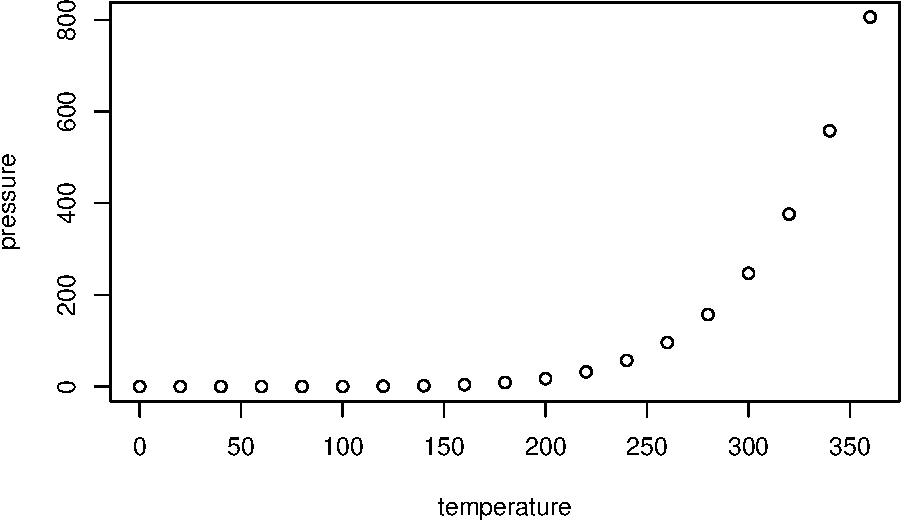
\includegraphics{manuscript_files/figure-latex/plot-1.pdf}

You can also mix text and code, so called inline code, like this: 7.

Discussion

Conclusion

References

\hypertarget{refs}{}
\begin{CSLReferences}{0}{0}
\leavevmode\vadjust pre{\hypertarget{ref-GBD_2017_Causes_of_Death_Collaborators2018-oe}{}}%
\CSLLeftMargin{1. }
\CSLRightInline{GBD 2017 Causes of Death Collaborators. Global,
regional, and national age-sex-specific mortality for 282 causes of
death in 195 countries and territories, 1980-2017: A systematic analysis
for the global burden of disease study 2017. Lancet. 2018
Nov;392(10159):1736--88. }

\leavevmode\vadjust pre{\hypertarget{ref-Candefjord2022-pe}{}}%
\CSLLeftMargin{2. }
\CSLRightInline{Candefjord S, Asker L, Caragounis E-C. Mortality of
trauma patients treated at trauma centers compared to non-trauma centers
in sweden: A retrospective study. Eur J Trauma Emerg Surg. 2022
Feb;48(1):525--36. }

\leavevmode\vadjust pre{\hypertarget{ref-Drake2020-kx}{}}%
\CSLLeftMargin{3. }
\CSLRightInline{Drake SA, Holcomb JB, Yang Y, Thetford C, Myers L, Brock
M, et al. Establishing a regional trauma preventable/potentially
preventable death rate. Ann Surg. 2020 Feb;271(2):375--82. }

\leavevmode\vadjust pre{\hypertarget{ref-Ray2016-jo}{}}%
\CSLLeftMargin{4. }
\CSLRightInline{Ray JJ, Meizoso JP, Satahoo SS, Davis JS, Van Haren RM,
Dermer H, et al. Potentially preventable prehospital deaths from motor
vehicle collisions. Traffic Inj Prev. 2016 Oct;17(7):676--80. }

\leavevmode\vadjust pre{\hypertarget{ref-Ghorbani2018-dh}{}}%
\CSLLeftMargin{5. }
\CSLRightInline{Ghorbani P, Strömmer L. Analysis of preventable deaths
and errors in trauma care in a scandinavian trauma level-i centre. Acta
Anaesthesiol Scand. 2018 Sep;62(8):1146--53. }

\leavevmode\vadjust pre{\hypertarget{ref-Kadhum2020-wa}{}}%
\CSLLeftMargin{6. }
\CSLRightInline{Kadhum M, Sinclair P, Lavy C. Are primary trauma care
({PTC}) courses beneficial in low- and middle-income countries - a
systematic review. Injury. 2020 Feb;51(2):136--41. }

\leavevmode\vadjust pre{\hypertarget{ref-Granstrom2012}{}}%
\CSLLeftMargin{7. }
\CSLRightInline{Granström A, Wihlke G, Brattström O, Ostlund A.
{{[}{A}ctivation of the trauma team is related to injury severity.
{T}riage stringency can yield optimal use of resources{]}}.
Lakartidningen. 2012;109(4):154--7. }

\end{CSLReferences}

\end{document}
